\documentclass[a4paper, 12pt]{article}
\usepackage{amsmath, amssymb, amsthm, stmaryrd}
\usepackage{geometry}
\usepackage{tcolorbox}
\usepackage{pgfplots}
\usepackage{hyperref}

\geometry{hmargin=2.5cm, vmargin=2.5cm}

\renewcommand*{\today}{06 December 2024}

\title{Analyse}
\author{Par Lorenzo}
\date{\today}

\newtheorem{theorem}{Théorème}[section]
\newtheorem{definition}{Définition}[section]
\newtheorem{example}{Example}[section]
\newtheorem{remark}{Remarques}[section]
\newtheorem{lemme}{Lemme}[section]
\newtheorem{corollaire}{Corollaire}[section]

\newtheorem{_proposition}{Proposition}[section]
\newenvironment{proposition}[1][]{
    \begin{_proposition}[#1]~\par
    \vspace*{0.5em}
}{%
    \end{_proposition}%
}

\newtheorem{_proprietes}{Propriétés}[section]
\newenvironment{proprietes}[1][]{
        \begin{_proprietes}[#1]~\par
        \vspace*{0.5em}
}{%
        \end{_proprietes}%
}

\newenvironment{rdem}[1][]{
    \begin{tcolorbox}[colframe=black, colback=white!10, sharp corners]
        #1
}{%
    \end{tcolorbox}
     
}

\newtheorem{_demonstration}{Démonstration}[section]
\newenvironment{demonstration}[1][]{
    \begin{_demonstration}[#1]~\par
    \vspace*{0.5em}
}{%
    \end{_demonstration}%
    \qed%
}

\newtheorem*{_demonstration*}{Démonstration}
\newenvironment{demonstration*}[1][]{
    \begin{_demonstration*}[#1]~\par
    \vspace*{0.5em}
}{%
    \end{_demonstration*}%
    \qed%
}

\newenvironment{ldefinition}{
    \begin{definition}~\par
    \vspace*{0.5em}
    \begin{enumerate}
}{
        \end{enumerate}
        \end{definition}
}

\newenvironment{lexample}{
    \begin{example}~\par
    \vspace*{0.5em}
    \begin{enumerate}
}{
        \end{enumerate}
        \end{example}
}

\newtheorem{_methode}{Méthode}[section]
\newenvironment{methode}{
    \begin{_methode}~\par
    \vspace*{0.5em}
}{
        \end{_methode}
}

\def\N{\mathbb{N}}
\def\Z{\mathbb{Z}}
\def\Q{\mathbb{Q}}
\def\R{\mathbb{R}}
\def\C{\mathbb{C}}
\def\K{\mathbb{K}}
\def\k{\Bbbk}

\def\un{(u_n)_{n \in \N}}
\def\xn#1{(#1_n)_{n \in \N}}

\def\o{\overline}
\def\eps{\varepsilon}

% \funcdef{name}{domain}{codomain}{variable}{expression}
% name: Name of the function (e.g. f)
% domain: Domain of the function (e.g. \mathbb{R})
% codomain: Codomain of the function (e.g. \mathbb{R})
% variable: Variables of the function (e.g. x)
% expression: Expression of the function (e.g. x^2)
\newcommand{\funcdef}[5]{%
    #1 :
    \begin{cases}
        #2 \rightarrow #3 \\
        #4 \mapsto #5
    \end{cases}
}

\newcommand{\lt}{\ensuremath <}
\newcommand{\gt}{\ensuremath >}

\begin{document}

\maketitle

\tableofcontents


% Begin of 2024-09-12-CM-1.tex

\section{L'ensemble des nombres rationnels $\Q$}

\subsection{Ecriture décimale}

\begin{definition}
    On definit l'ensemble des nombres rationnels $\Q$ par \break
    $\Q = \{\dfrac{p}{q} \mid p \in \Z, q \in \N^*\}$,
    optionellement $pgcd(p, q) = 1$ peut être rajouté dans la définition.
    Cela ajoute le fait que p et q sont premier entre eux et donc $\dfrac{p}{q}$ un fraction irréductible.
    (rappel: $\N^*=\N\backslash\{0\}$, i.e. $\N$ privé de 0).
\end{definition}

\begin{remark}
    Les nombres décimaux sont des nombres de la forme \break $\dfrac{p}{10^n}$ avec $p \in \Z, n \in \N$
    (e.g. $1.234 = \dfrac{1234}{10^3}$).
\end{remark}

\begin{proposition}
    Un nombre est rationnel si et seulement si il admet une écriture décimale finie ou périodique.
\end{proposition}

\begin{demonstration}
    Démontrons que si un nombre à une partie décimale finie ou périodique, alors il est rationnel.

    \vspace{1em}

    a) partie décimale finie

    \vspace{0.5em}

    1. Supposons que x soit un nombre réel avec une partie décimale finie.
    x peut s'écrire sous la forme:
    \begin{align*}
        x = a.b_1b_2...b_n
    \end{align*}
    Ou $a \in \Z$ est la partie entière et $b_1b_2...b_n$ avec $n \in \N$ représente les chiffres de la partie décimale finie.
    
    \vspace{0.5em}

    2. On peut écrire x comme:
    \begin{align*}
        x = a + \dfrac{b_1b_2...b_n}{10^n}
    \end{align*}

    Ici, a est un entier et $\dfrac{b_1b_2...b_n}{10^n}$ un nombre rationnel.

    \begin{rdem}
        La somme d'un entier (nombre rationnel) et d'un nombre rationnel est un nombre rationnel.
    \end{rdem}

    \vspace{1em}

    b) partie décimale périodique

    \vspace{0.5em}

    1. Supposons que x soit un nombre réel avec une partie décimale périodique.
    x peut s'écrire sous la forme:
    \begin{align*}
        x = a.b_1b_2...b_n\overline{c_1c_2...c_m}
    \end{align*}
    où $a \in \Z$ est la partie entière, $b_1b_2...b_n$ sont les chiffres non répétitifs initiaux, et
    $\overline{c_1c_2...c_m}$ est le bloc périodique.

    \vspace{0.5em}

    2. Pour simplifier la démonstration, on peut isoler la partie périodique. Posons:
    \begin{align*}
        y = 0.\overline{c_1c_2...c_m}
    \end{align*}
    \vspace{0.5em}
    
    3. On multiplie y par $10^m$, où m est la longeur de la période.
    \begin{align*}
        &10^m y = c_1c_2...c_m + y \\
        \iff& 10^m y - y = c_1c_2...c_m \\
        \iff& y(10^m - 1) = c_1c_2...c_m \\
        \iff& y = \dfrac{c_1c_2...c_m}{10^m - 1} \\
    \end{align*}
    y est donc rationnel.

    \vspace{0.5em}

    4. On peut réexprimer x
    \begin{align*}
        x = a + \dfrac{b_1b_2...b_n}{10^n} + y
    \end{align*}

    \begin{rdem}
        La somme de nombre rationnel donne un nombre rationnel.
    \end{rdem}
    
    \begin{rdem}
        Ainsi si un nombre à une partie décimale finie ou périodique, alors il est rationnel.
    \end{rdem}


\end{demonstration}

\begin{demonstration}
    Démontrons que si un nombre est rationnel, alors sa partie décimale est finie ou périodique.

    Supposons que x est un nombre rationnel ainsi il s'écrit sous la forme
    $x = \dfrac{p}{q}$ avec $p \in \Z \text{ et } q \in \N^*$

    Lorsque qu'on effectue la division euclidienne $\dfrac{p}{q}$ deux cas se présentent:

    La division se termine par un nombre fini d'étapes.

    La division ne se termine pas et répète une séquence de chiffres.

    \begin{rdem}
        Ainsi si un nombre est rationnel, alors sa partie décimale est finie ou périodique.
    \end{rdem}

\end{demonstration}

\begin{example}
    Prenons $x = 12.34202320232023...$

    \vspace{1em}

    Etape 1: faire apparaitre la partie périodique à la virgule.
    Ici on multiplie par 100
    \begin{flalign}
        100x = 1\,234.202320232023...&&
    \end{flalign}
    Etape 2: on décale d'une période vers la gauche.
    Ici la période est de longeur 4 donc on multiplie par 10 000.
    \begin{flalign}
        10\,000 \times 100x = 12\,342\,023.20232023...&&
    \end{flalign}
    Etape 3: on soustrait (2) par (1) pour que la partie décimale s'annule.
    \begin{flalign}
        &10\,000 \times 100x - 100x = 12\,342\,023 - 1\,234&& \\
        \iff &999\,900x = 12\,340\,789&& \\
        \iff &x = \dfrac{12\,340\,789}{999\,900}&& \\
    \end{flalign}
\end{example}


% End of 2024-09-12-CM-1.tex

% Begin of 2024-09-12-CM-2.tex

\section{$\sqrt{2}$ n'est pas un rationnel}

Il existe des nombres qu'on ne peut pas écrire sous la forme d'une fraction de deux entiers, on les nomme les irrationnels.
Ils apparaissent naturellement (e.g. La diagonale d'un carré de longeur 1).

\begin{proposition} \label{propal}
    Pour la suite nous avons besoin de démontrer que 
    \begin{align*}
        p \in \Z, \; 2 \mid p^2 \implies 2 \mid p
    \end{align*}

    si $p^2$ est pair alors $p$ est pair

\end{proposition}

\begin{demonstration}
    Supposons que le carré d'un nombre impair est pair:

    \begin{align*}
        \forall k \in \Z, \; p = 2k + 1 \quad \iff \quad p^2 =&\; (2k + 1)^2 \\
         =&\; (2k)^2 + 2*2k*1 + 1^2 \\
         =&\; 4k^2 + 4k + 1 \\
         =&\; 2(2k^2 + 2k) + 1
    \end{align*}

    
    Ici $p^2$ est impair, Absurde $p^2$ ne peut pas être à la fois pair et impair!
    \begin{rdem}
        Donc si le carré d'un entier relatif $(p^2)$ est pair p est aussi pair.
    \end{rdem}

\end{demonstration}

\begin{proposition}
    $\sqrt{2} \in \R \backslash \Q$ ($\sqrt{2}$ est irrationnel).
\end{proposition}

\begin{demonstration}
    Supposons que $\sqrt{2}$ est un rationnel, c'est à dire,
    
    \begin{align*}
        \exists \; p \in \Z, q \in \N^*, \; pgcd(p, q) = 1, \quad \sqrt{2}=\dfrac{p}{q}
    \end{align*}

    Ici, $pgcd(p, q) = 1$ signifie que $p$ et $q$ sont premiers entre eux. Cette condition est importante pour assurer que la fraction est irréductible.


    \begin{align*}
        \sqrt{2} = \dfrac{p}{q} \quad \iff& \quad 2 = \dfrac{p^2}{q^2} \\
        \iff& \quad p^2 = 2q^2
    \end{align*}

    \vspace{0.5em}
    %todo check pourquoi \ref{propal} fait de la demer
    Ici on peut voir que $p^2$ est pair et grace à \textbf{(la proposition 1.1)} on sait que $p$ l'est aussi.
    Donc on peut réecrire $p$ par $\exists k \in \Z, \; 2k = p$
    et ainsi remplacer $p^2$.

    \nobreak

    \begin{align*}
        2q^2 = p^2 \quad \iff& \quad 2q^2 = (2k)^2 \\
        \iff& \quad q^2 = \dfrac{4p^2}{2} \\
        \iff& \quad q^2 = 2p^2
    \end{align*}

    Donc $q^2$ est pair et $q$ également.

    Finalement 2 divise p et q est absurde car p et q sont premier entre eux, ils ne peuvent pas être tout les deux multiple de 2.
    
    \begin{rdem}
        L'hypothèse de départ $\sqrt{2} \in \R \backslash \Q$ est fausse, ainsi $\sqrt{2}$ est irrationnel.
    \end{rdem}

\end{demonstration}

\section{Propriété de $\R$}

On nomme $\R$ l'ensemble des nombres réels, il contient $\N$, $\Z$, $\Q$ et $\R \backslash \Q$.

$\overline{\R} = \R \cup \{-\infty; +\infty\}$ (les réels et l'infini)

\subsection{Règle de calcul}

Soient a, b et c des nombres réels quelconques.
On note $+$ l'addition et $\times$ la multiplication.

\vspace*{1em}

\begin{proprietes}
    \item l'associativité.
        \begin{flalign*}
            &(a + b) + c = a + (b + c)&& \\
            &(a \times b) \times c = a \times (b \times c)&&
        \end{flalign*}
    \item l'élement neutre.
        \begin{flalign*}
            &\exists e \in \R, \forall x \in \R, \; e + x = x + e = x&& \\
            &\exists e' \in \R, \forall x \in \R, \; e' \times x = x \times e' = x&&
        \end{flalign*}
        Pour l'addition et la multiplication dans $\R$, leur élément neutre est 0 et 1 respectivement.
        e et e' seront pour la suite, les élements neutres de l'addition et de la multiplication respectivement.
    \item l'élement inverse.
        \begin{flalign*}
            &\exists i \in \R, \forall x \in \R, \; i + a = a + i = e&& \\
            &\exists i \in \R^*, \forall x \in \R^*, \; i \times a = a \times i = e'&&
        \end{flalign*}
    \item commutativité.
        \begin{flalign*}
            &a + b = b + a&& \\
            &a \times b = b \times a&&
        \end{flalign*}
    \item distributivité de la multiplication par rapport à l'addition.
    \begin{flalign*}
        &(a + b) \times c = c \times (a + b) = ac + bc&& \\
    \end{flalign*}
\end{proprietes}

\begin{remark}
    $(\R, +, *)$ est un corps abélien/commutatif
\end{remark}

\subsection{L'ordre sur $\R$}

Soient a, b et c des nombres réels quelconques.

\begin{proprietes}
    \item réfléxivité.
        \begin{flalign*}
            a \leq a
        \end{flalign*}
    \item l'antisymmétrie.
        \begin{flalign*}
            a \leq b \text{ et } b \leq a \implies a = b
        \end{flalign*}
    \item transitivité.
        \begin{flalign*}
            a \leq b \text{ et } b \leq a \implies a = b
        \end{flalign*}
    \item comparabilité
    
        quelque soit a et b dans $\R$, on a toujours $a \leq b$ or $b \leq a$
\end{proprietes}

\noindent
Les propriétés 1, 2 et 3 signifie que $leq$ est une relation d'ordre,
ajouté la 4, on parle de relation d'ordre totale.

\begin{remark}
    On définit la relation d'ordre supérieur ou égale ($\geq$) par \break $a \geq b \iff b \leq a$
\end{remark}

\begin{remark}
    On définit la relation d'ordre strictement inférieur ($\lt$) par \break $a \lt b \iff a \leq b \text{ et } a \neq b$
\end{remark}

\begin{remark}
    On définit la relation d'ordre strictement supérieur ($\gt$) par \break $a \gt b \iff a \geq b \text{ et } a \neq b$
\end{remark}

\begin{remark}
    $\lt$ et $\gt$ ne vérifient pas 1 et 2, ils ne sont donc pas des relations d'ordres mais des relations d'ordres stricts.
\end{remark}

\begin{proprietes}
    \item $a \leq b \implies a + c \leq b + c$
    \item $a \leq b \text{ et } c \geq 0 \implies ac \leq bc$
    \item $ab = 0 \implies a = 0 \text{ ou } b = 0$
\end{proprietes}

On définit le maximum entre deux réels comme
\begin{equation*}
    max(a, b) =
    \begin{cases}
        a, & \text{si } b \leq a \\
        b, & \text{sinon}
    \end{cases}
\end{equation*}


% End of 2024-09-12-CM-2.tex

% Begin of 2024-09-19-CM-3.tex

\subsection{Propriété d'Archimède}

L'ensemble $\R$ est dit archimédien, i.e. $\forall x \in \R, \exists n \in \N, \; x \lt n$

\begin{proposition}
    Il existe un unique entier dans $\Z$, appelé la partie entière E, tel que $E(x) \leq E(x) + 1$
\end{proposition}

\begin{demonstration}
    \textbf{Existence:} Supposons que $x \geq 0$.
    Comme $\R$ est archimédien il existe un entier $n \in \N$ tel que $x \lt n$.

    \begin{rdem}
        Ainsi on peut trouver un autre entier $m \in \N$ tel que $n \leq x$ et $m \lt n$.
        Il suffit de choisir m comme le plus grand entier inférieur ou égal à x et tel que $m \leq x \lt m + 1$
    \end{rdem}

    \vspace{1em}

    \noindent
    \textbf{Unicité:} Supposons qu'il existe 2 entiers tel que $k \leq x \lt k + 1$ et $l \leq x \lt l + 1$

    Par transitivité, il vient $k \leq x \lt l + 1$ et $k \lt l + 1$,

    de même, $l \leq x \lt k + 1$ et $l \lt k + 1 \implies l - 1 \lt k$

    \begin{rdem}
        Finalement $l - 1 \lt k \lt l + 1$ et comme entre les entiers l'entier l-1 et l+1 il n'y a que l, alors k = l
    \end{rdem}
\end{demonstration}

\begin{example}
    \item x = 3.14, E(x) = 3.
    \item x = -12.2, E(x) = -13.
\end{example}

\begin{remark}
    \item On note parfois $E(x) = [x] = \lfloor x \rfloor$
    \item On note $\{x\}$, la partie fractionnaire (e.g. $\{3.14\}=0.14$)
\end{remark}

% \begin{tikzpicture}
%     \begin{axis}[axis lines=middle, grid]
%         \addplot[
%             jump mark right,
%             domain=-3:3,
%             samples=7,
%             very thick, red,
%         ]{floor(x)};
%         \addlegendentry{\(E(x)\)};
%     \end{axis}
% \end{tikzpicture}

% \begin{tikzpicture}
%     \begin{axis}[axis lines=middle, grid, ymin=-3, ymax=3]
%         \addplot[
%             jump mark right,
%             domain=-3:3,
%             samples=1000,
%             very thick, red,    
%         ]{x-floor(x)}; 
%         \addlegendentry{$\{x\}$};
%     \end{axis}
% \end{tikzpicture}

\includegraphics[width=\textwidth]{images/Entier&fractionaire.png}

\subsection{La valeur absolue}

\begin{definition}
    Soit x un nombre réel. La valeur absolue de x est le nombre réel positif défini par
    \begin{equation}
        |x| =
        \begin{cases}
            x, & \text{si } x \geq 0 \\
            -x, & \text{si } x \lt 0
        \end{cases}
    \end{equation}
\end{definition}

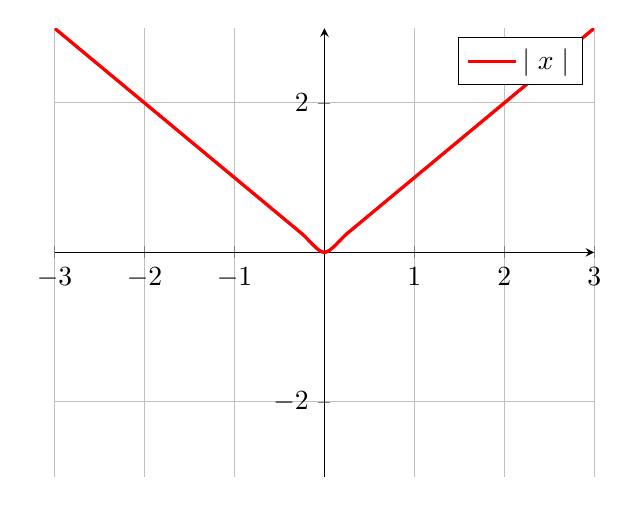
\begin{tikzpicture}
    \begin{axis}[axis lines=middle, grid, ymin=-3, ymax=3]
        \addplot[
            jump mark right,
            domain=-3:3,
            smooth,
            very thick, red,    
        ]{abs(x)}; 
        \addlegendentry{$\mid x \mid$};
    \end{axis}
\end{tikzpicture}

\noindent
Soient $a, b, c \in \R$

\begin{proprietes}
    \item $|a| \geq 0, \quad a \leq |a|, \quad -|a| \leq a, \quad |-a| = |a|$
    \item $\sqrt{a^2} = |a|$
    \item $|ab| = |a||b|$
    \item $\forall n \in \Z, |a^n| = |a|^n$
    \item $\text{si } a \neq 0, |\dfrac{1}{a}|=\dfrac{1}{|a|} \text{ et } |\dfrac{b}{a}| = \dfrac{|b|}{|a|}$
    \item
        $\text{Pour } b \geq 0,$
        
        $|a| = b, \text{ si et seulement si } a = b \text{ ou } a = -b$
        
        $|a| \leq b \text{ si et seulement si } -b \leq a \leq b$ (beaucoup utilisé pour passer de $a$ à $|a|$)

        $|a| \geq b \text{ si et seulement si } a \leq -b \text{ ou } a \geq b$
    \item $|a + b| \leq |a| + |b|$ (l'inégalité triangulaire)
    \item $||a| - |b|| \leq |a - b|$ (l'inégalité triangulaire inversée)
\end{proprietes}

Les propriétés 1 à 6 sont démontrés par la définition de la valeur absolue

Démontrons la proprétée 7.

\begin{demonstration}
    D'après (1) \quad
    $-|a| \leq a \leq |a|$ et $-|b| \leq b \leq |b|$
    
    En additionnant, on obtient $-|a|-|b| \leq a + b \leq |a| + |b|$

    $-(|a|+|b|) \leq a + b \leq |a| + |b|$ avec (6) on arrive à

    $|a + b| \leq |a| + |b|$
\end{demonstration}

Démontrons la propriétée 8.

\begin{demonstration}
    $a = a - b + b$ \quad et \quad $|a| = |a - b + b| \leq |a - b| + |b|$ (propriétée 7)

    $|a| \leq |a - b| + |b| \implies |a| - |b| \leq |a - b|$

    \vspace{0.5em}
    de même, 
    \vspace{0.5em}
    
    $b = b - a + a$ \quad et \quad $|b| = |b - a + a| \leq |b - a| + |a|$
    
    $|b| \leq |b - a| + |a| \implies |b| - |a| \leq |b - a|$
    
    \vspace{0.5em}

    $|b - a| = |-(a-b)| = |a-b|$ et
    
    $|a| - |b| \leq |a-b|$ \quad et \quad $|b| - |a| = -(|a| - |b|) \leq |a-b|$

    Finalement par définition

    \begin{rdem}
        \begin{equation*}
            ||a|-|b|| =
            \begin{cases}
                |a| - |b|, & \text{si } |a| - |b| \geq 0 \\
                -(|a| - |b|), & \text{si } |a| - |b| \lt 0
            \end{cases}
        \end{equation*}
        Ainsi $||a| - |b|| \leq |a - b|$
    \end{rdem}
\end{demonstration}

Corollaire: Soit r un réel positif $\forall x, a \in \R$, on a 
$|x - a| \lt r \implies -r \lt x - a \lt r \implies a-r \lt x \lt a + r$

\begin{remark}
    La valeur absolue $|b - a|$ représent la distance entre a et b
\end{remark}

\includegraphics[width=\textwidth]{images/neightborhood.png}

\section{Densité de $\Q$ dans $\R$}

\subsection{Intervalles de $\R$}

\begin{definition}
    On appelle intervalle de $\R$, tout sous-ensemble I de $\R$ vérifiant
    $\forall a, b \in I, a \leq b \text{ et } x \in \R, a \leq x \leq b \implies x \in I$
\end{definition}

\begin{remark}
    Un sous-ensemble ou partie I de $\R$, se note $I \subset \R$
\end{remark}

\begin{definition}
    Soient $a, b \in \R, a \leq b$

    On appelle intervalle fermé et borné (ou segment) de $\R$ tout l'ensemble de la forme

    $[a, b] = \{x \in \R | \; a \leq x \leq b\}$
    
    \vspace{0.5em}

    On appelle intervalle ouvert de $\R$ tout l'ensemble de la forme

    $]a, b[ = \{x \in \R | \; a \lt x \lt b\}$
    \quad ou \quad
    $]a, +\infty[ = \{x \in \R | \; a \lt x\}$
    \par ou \quad
    $]-\infty, b[ = \{x \in \R | \; x \lt b\}$
\end{definition}

\begin{remark}
    L'ensemble qui contient aucun élément est l'ensemble vide, noté $\emptyset$
\end{remark}

\begin{remark}
    L'ensemble qui contient un seul élément est le singleton, noté $\{a\} = [a, a]$
\end{remark}

\begin{remark}
    $x \in [a, b] \equiv \exists t \in [0, 1], x = (1-t)a + tb$
\end{remark}

\begin{definition}
    On dit que V est un voisinage de a si $\exists \epsilon \gt 0, \; [a - \epsilon, a + \epsilon] \subset V$
\end{definition}

\subsection{Densité}

\begin{theorem}
    $\Q$ est dense dans $\R$, tout intervalle ouvert, non vide de $\R$ contient une infinité de nombres rationnels
\end{theorem}
\begin{theorem}
    $\R \backslash \Q$ est dense dans $\R$, tout intervalle ouvert, non vide de $\R$ contient une infinité de nombres irrationnels
\end{theorem}

\begin{demonstration}
    On cherche $\dfrac{p}{q} \in \Q, p \in \Z, q \in \N^*$
    tel que $a \lt \dfrac{p}{q} \lt b \implies aq \lt p \lt bq$

    comme $\R$ est archimédien, il existe un entier q tel que $q \gt \dfrac{1}{b - a} \implies \dfrac{1}{q} \lt b - a$

    Prenons $p = E(aq) + 1$

    $p = E(aq) + 1 \implies p - 1 = E(aq) \leq aq \lt E(aq) + 1 = p$

    \vspace{0.5em}

    On divise par q l'inégalité $p - 1 \geq aq \lt p + 1$

    $\implies \dfrac{p-1}{q} = \dfrac{p}{q} - \dfrac{1}{q} \leq a \lt \dfrac{p}{q}$
    
    Ainsi
    $\dfrac{p}{q} - \dfrac{1}{q} \leq a \implies \dfrac{p}{q} \leq a + \dfrac{1}{q} \lt a + (b-a) = b$

    \begin{rdem}
        Finalement $a \lt \dfrac{p}{q} \lt b$

        Il existe un nombre rationnels $\dfrac{p}{q}$ compris entre a et b.
    \end{rdem}

    On divise l'intervalle $]a,b[$ en N sous-intervalles disjoints 2 à 2
    
    $]a, b[ = ]a, a+\dfrac{b-a}{N}[ \cup ]\dfrac{b-a}{N}, a + 2\dfrac{b-a}{N}[$

    \includegraphics{images/interval.png}

    \begin{rdem}
        Donc pour chaque intervalle on peut trouver un rationnels, on peut ensuite faire tendre N vers l'infini pour trouver un infinité de rationnels
    \end{rdem}
\end{demonstration}

\begin{demonstration}
    D'apres notre démonstration précédente il existe un infinité de rationnels pour

    $a - \sqrt{2} \lt \dfrac{p}{q} \lt b - \sqrt{2} \implies a \lt \dfrac{p}{q} + \sqrt{2} \lt b$

    \begin{rdem}
        On en arrive avec la même logique que la démonstration précédente qu'il existe une infinité d'irrationnels entre deux réels.
    \end{rdem}
\end{demonstration}
        
\section{Bornes sur $\R$}

\subsection{Maximum et minimum}

\begin{definition}
    Soit A une partie non vide de $\R$. Un réel M est le plus grand (resp. le plus petit) élément de A si $M \in A$ et
    $\forall x \in A, x \leq M$ (resp. $\forall x \in A, x \geq m$).

    Si il existe, le plus grand élément est unique et on le note max A.

    Si il existe, le plus petit élément est unique et on le note min A.
\end{definition}


% End of 2024-09-19-CM-3.tex

% Begin of 2024-09-26-CM-4.tex

\subsection{Majorants et minorants}

\begin{definition}
    Soit A une partie non vide de $\R$, un réel M est dit majorant de A si il vérifie $\forall x \in A, \; M \geq x$
\end{definition}

\begin{definition}
    Soit A une partie non vide de $\R$, un réel m est dit minorant de A si il vérifie $\forall x \in A, \; m \leq x$
\end{definition}

\begin{remark}
    Le majorant et minorant n'appartiennent pas forcément à l'ensemble A.
\end{remark}

\begin{definition}
    Si un majorant (resp. minorant) de A existe, on dit que A est majorée (resp. minorée). On dit que A est bornée si A est majorée et minorée.
\end{definition}

\subsection{Bornes supérieures et bornes inférieures}

\begin{definition}
    Soit A un partie non vide de $\R$.

    \item \textbf{1.} On dit que M est la borne supérieure de A, si M est un majorant de A et que M est le plus petit des majorants.
        Si il existe on note M = sup A.
    \item \textbf{2.} On dit que m est la borne inférieure de A, si m est un minorant de A et que m est le plus grand des minorant.
        Si il existe on note m = inf A.
\end{definition}

\begin{remark}
    sup A et inf A n'appartiennent pas forcément à A. Mais si ils appartiennent à l'ensemble ils deviennent max A et min A respectivement.
\end{remark}

\begin{example}
    Posons $A := [0, 1[$,

    $min A = 0$ et $max A$ n'existe pas.

    les minorants de A sont $]-\infty, 0]$ et les majorants de A sont $[1, +\infty[$
    
    $inf A = 0$ et $sup A = 1$
\end{example}

\begin{proposition}
    Soit A une partie non vide de $\R$ et majorée. La borne supérieure est l'unique réel sup A, tel que
    
    \item (i)$\forall x \in A, \; x \leq sup A$ et
    \item (ii) $\forall y \in \R, \; y \lt sup A \implies (\exists x \in A, y \lt x)$
\end{proposition}

\begin{demonstration}
    Montrons que sup A vérifie (i) et (ii).

    \begin{rdem}
        Comme sup A est un majorant, elle vérifie (i)
    \end{rdem}

    Posons $y \lt sup A$, comme sup A est le plus petit des majorants, y ne peut pas être un majorant de A.
    
    \begin{rdem}
        Donc $\exists x \in A, \; y < x$
    \end{rdem}

    Soit M un réel qui vérifie (i) et (ii), supposons que M n'est pas le plus petit des majorants.
    Il existe un autre majorant y, tel que $y \lt M$.

    \begin{rdem}
        Mais d'après (ii) $\exists x \in A, \; y < x$, donc y n'est pas un majorant de A.
    \end{rdem}
\end{demonstration}

\begin{theorem}
    Toute partie non vide de $\R$ majorée admet une borne supérieure.
\end{theorem}

\begin{theorem}
    Toute partie non vide de $\R$ minorée admet une borne inférieure.
\end{theorem}

\begin{proposition}
    Soit A une partie non vide majorée de $\R$. La borne supérieure est l'unique réel sup A, tel que

    \item (i) sup A est un majorant de A
    \item (ii) il existe une suite $(x_n)_{n \in \N}$ d'éléments de A qui converge vers sup A.
\end{proposition}

\section{Les suites}

\subsection{Définition d'une suite}

\begin{definition}
    Une suite est l'application
    \begin{align*}
        u: \N &\longrightarrow \R\\
        n &\longmapsto u(n)
    \end{align*}
    Pour $n \in \N$, on note $u(n)$, ou plus souvent $u_n$, le n-ième terme de la suite.
    On écrit~$(u_n)_{n \in \N}$
\end{definition}


% End of 2024-09-26-CM-4.tex

% Begin of 2024-10-03-CM-5.tex

\begin{example}
    \item $\bullet$ $(n)_{n \in \N}$ est la suite des entiers.
    \item $\bullet$ $((-1)^n)_{n \in \N}$ est la suite alternant entre 1 et -1.
    \item $\bullet$ $(F_n)_{n \in \N}$ définie par $F_0=1, F_1=1, F_{n+2}=F_{n+1}+F_n$
    est la suite de Fibonacci.
\end{example}

\begin{remark}
    Ne pas confondre la fonction avec une suite ($(\sqrt{n})_{n \in \N}$ différent de $f(x)= \sqrt{x}$)
\end{remark}

\subsubsection{Suites majorées, minorées, bornées}

\begin{definition}
    Soit $\un$ une suite de nombre réels.
    
    \item On dit que la suite $\un$ est
    \textbf{majorée} si $\exists M \in \R, \forall n \in \N, u_n \leq M$.
    
    \item On dit que la suite $\un$ est
    \textbf{minorée} si $\exists M \in \R, \forall n \in \N, M \leq u_n$.

    \item On dit que la suite $\un$ est
    \textbf{bornée} si la suite $\un$ est majorée et minorée.\par
    (i.e. $\exists M \in \R, \forall n \in \N, |u_n| \leq M$)
\end{definition}

\begin{definition}
    \item La suite $\un$ est \textbf{croissante} si $\forall n \in \N, u_{n+1} \geq  u_n$.
    
    \item La suite $\un$ est \textbf{strictement croissante} si $\forall n \in \N, u_{n+1} \gt  u_n$.
    
    \item La suite $\un$ est \textbf{décroissante} si $\forall n \in \N, u_{n+1} \leq  u_n$.

    \item La suite $\un$ est \textbf{strictement décroissante} si $\forall n \in \N, u_{n+1} \lt  u_n$.

    \item On dit que la suite est \textbf{monotone} si elle est croissante ou décroissante.
\end{definition}

\begin{remark}
    Pour vérifier la monotonie d'une suite:

    \item Soit $u_{n+1} - u_n \geq 0 \implies$ croissante
    \item Soit on calcule (avec $u_n \neq 0$) $\dfrac{u_{n+1}}{u_n} \geq 1 \implies$ croissante

    On préfère la première pour les suites arithmétiques et la deuxième pour les suites géométriques.
\end{remark}

\subsection{Limites}

\subsubsection{Limit finie, limite infinie}

\begin{definition}
    La suite $\un$ admet pour limite $l \in \R$ si
    $$
    \forall \varepsilon \gt 0, \exists N \in \N, \forall n \geq N, |u_n - l| \leq \varepsilon
    $$

    On dit que la suite $\un$ tend vers l quand n tend vers l'infini, ou
    $$
    \lim_{n \to \infty} u_n = l
    $$
\end{definition}

\includegraphics{images/limite.png}

\begin{remark}
    On utilise $\varepsilon$ pour parler d'un nombre très petit.
\end{remark}

\begin{definition}
    La suite $\un$ tend vers $+\infty$ si elle devient aussi grande que l'on souhaite quand n
    devient grand, autrement dit

    $$
    \forall A \gt 0, \exists N \in \N, \forall n \geq N, u_n \geq A
    $$

    La suite $\un$ tend vers $-\infty$ si elle devient aussi petite que l'on souhaite quand n
    devient grand, autrement dit

    $$
    \forall A \gt 0, \exists N \in \N, \forall n \geq N, u_n \leq -A
    $$
\end{definition}

\begin{definition}
    \item $\un$ \textbf{converge} si elle admet une limite finie.

    \item $\un$ \textbf{diverge} si elle admet l'infini comme limite ou si elle n'a pas de limite.
\end{definition}

\begin{proposition}
    Si une suite converge, alors sa limite est unique.
\end{proposition}

\begin{demonstration}
    Soit $\un$ une suite qui admet deux limite, $l_1 \neq l_2$.
    
    $$
    \lim_{n \to +\infty}u_n = l_1 \implies
    \forall \varepsilon_1, \exists N_1 \in \N, \forall n \geq N_1, |u_n - l_1| \leq \varepsilon_1
    $$
    
    $$
    \lim_{n \to +\infty}u_n = l_2 \implies
    \forall \varepsilon_2, \exists N_2 \in \N, \forall n \geq N_2, |u_n - l_2| \leq \varepsilon_2
    $$

    Pour $\varepsilon_1 = \varepsilon = \varepsilon_2 \gt 0$
    
    $\exists N = max(N_1, N_2), \forall n \geq \N, |u_n - l_1| \lt \varepsilon \text{ et } |u_n - l_2| \lt \varepsilon$

    Donc $|l_1 - l_2| = |l_1 - u_n + u_n - l_2| = |(l_1 - u_n) + (u_n - l_2)| \leq |l_1 - u_n| + |u_n - l_2| \lt \varepsilon + \varepsilon = 2 \varepsilon$

    Il suffit de prendre $\varepsilon \lt \dfrac{|l_1 - l_2|}{2}$, ainsi

    $$
    |l_1 - l_2| \lt 2\varepsilon \leq |l_1 - l_2|
    $$

    \begin{rdem}
        Ce qui est absurde, Finalement $l_1 = l_2$
    \end{rdem}
\end{demonstration}

\subsubsection{Propriétés des limites}

\begin{proprietes}
    \item $\lim_{n \to +\infty} u_n = l \iff \lim_{n \to +\infty}(u_n - l) = 0 \iff \lim_{n \to +\infty} |u_n - l| = 0$
    \item $\lim_{n \to +\infty} u_n = l \implies \lim_{n \to +\infty}|u_n| = |l|$
\end{proprietes}

\begin{remark}
    C'est en général faux dans l'autre sens. Par exemple pour $u_n = (-1)^n$,
    $|u_n|=1$ donc $\lim_{n \to \infty} |u_n| = 1$ mais $\un$ n'a pas de limite (-1, 1, -1, 1, ...).
\end{remark}

\begin{proposition}
    Soient $\un$ et $\xn{v}$ deux suites convergentes.

    \item
    $$
    \lim_{n \to +\infty} u_n = l \implies \forall \delta \in \R, \lim_{n \to +\infty}(\delta u_n) = \delta l
    $$
    
    \item
    $$
    \lim_{n \to +\infty} u_n = l \text{ et } \lim_{n \to +\infty} v_n = l' \implies \lim_{n \to +\infty}(u_n + v_n) = l + l' \text{ et } \lim_{n \to +\infty}(u_n \times v_n) = l \times l'
    $$
    
    \item
    $$
    \exists N \in \N, \forall n \in \N, n \geq N, l \neq 0 \text{ et } u_n \neq 0 \implies \lim_{n \to +\infty} \dfrac{1}{u_n}=\dfrac{1}{l}
    $$
\end{proposition}

\begin{demonstration}

    \begin{align*}
        \lim_{n \to +\infty} u_n = l &\implies \forall \varepsilon \gt 0, \exists N \in \N, n \geq N, |u_n - l| \leq \varepsilon \\
        &\implies \forall \varepsilon \gt 0, \exists N \in \N, n \geq N, |\delta|| u_n - l|  \leq |\delta|\varepsilon \\
        &\implies \forall \varepsilon' \gt 0, \exists N \in \N, n \geq N, |\delta u_n - \delta l|  \leq |\delta|\varepsilon = \varepsilon' \\
        &\implies \lim_{n \to +\infty} \delta u_n = \delta l 
    \end{align*}

    \begin{align*}
        \lim_{n \to +\infty} u_n = l \implies \forall \varepsilon \gt 0, \exists N \in \N, n \geq N, |u_n - l| \leq \varepsilon \\
        \lim_{n \to +\infty} v_n = l' \implies \forall \varepsilon \gt 0, \exists N \in \N, n \geq N, |v_n - l'| \leq \varepsilon \\
        |u_n - l| + |v_n - l'| \geq |u_n - l + v_n - l'| = |(u_n + v_n) - (l + l')| \\
        \implies |(u_n + v_n) - (l + l')| \leq 2 \varepsilon = \varepsilon'
    \end{align*}

    \color{red}
    À compléter
    \color{black}
    \begin{align*}
        \lim_{n \to +\infty} u_n &= l \implies \forall \varepsilon \gt 0, \exists N \in \N, n \geq N, |u_n - l| \leq \varepsilon \\
        \lim_{n \to +\infty} v_n &= l' \implies \forall \varepsilon \gt 0, \exists N \in \N, n \geq N, |v_n - l'| \leq \varepsilon \\
        |u_n \times v_n - l \times l'| &= |u_n \times v_n - l \times v_n + l \times v_n - l \times l'| \\
        &= |v_n (u_n - l) + l (v_n - l')| \\
        &\leq |v_n (u_n - l)| + |l (v_n - l')| \\
        &= |v_n| |u_n - l| + |l| |v_n - l'|\\
    \end{align*}

    \color{red}
    À faire
    \color{black}
    \begin{align*}
        \lim_{n \to +\infty} u_n = l &\implies \forall \varepsilon \gt 0, \exists N \in \N, n \geq N, |u_n - l| \leq \varepsilon \\
    \end{align*}

\end{demonstration}


% End of 2024-10-03-CM-5.tex

% Begin of 2024-10-10-CM-6.tex

\begin{proprietes}
    Soient $\un$ et $\xn{v}$, tel que $lim_{n \to +\infty}v_n = +\infty$
    
    \item $$
    \lim_{n \to +\infty}\frac{1}{v_n} = 0
    $$

    \item Si $\un$ est minorée, alors
    $$
    \lim_{n \to +\infty}(u_n + v_n) = +\infty
    $$

    \item Si $\un$ est minorée par un réel strictement positif, alors
    $$
    \lim_{n \to +\infty}(u_n \times v_n) = +\infty
    $$

    \item Si $\lim_{n \to +\infty} u_n = 0$ et $\forall n \in \N, u_n \gt 0$, alors
    $$
    \lim_{n \to +\infty}\frac{1}{u_n} = +\infty
    $$
\end{proprietes}

\begin{theorem}
    Toute suite convergente est bornée.
\end{theorem}

\begin{demonstration}
    Soit une suite $\un$ qui converge vers l.

    $$
    \lim_{n \to +\infty}u_n = l \iff \forall \varepsilon \gt 0, \exists N \in \N, \forall n \in \N, n \geq N, |u_n - l| \lt \varepsilon
    $$

    On écrit $u_n = u_n - l + l$ ainsi $|u_n| = |(u_n - l) + l| \leq |u_n - l| + |l|$

    En outre $\forall n \geq N, |u_n| \leq \varepsilon + |l|$

    De plus $\forall n \lt N, |u_n| \leq \max(u_0, u_1, ..., u_{n-1})$

    \begin{rdem}
        Finalement $\forall n \in \N, |u_n| \leq \max(u_0, u_1, ..., u_{n-1}, \varepsilon + |l|)$
    \end{rdem}
\end{demonstration}

\begin{corollaire}
    Si la suite $\un$ est bornée et $\lim_{n \to \infty} v_n = 0$ alors $\lim_{n \to \infty} (u_n \times v_n) = 0$
\end{corollaire}

\subsubsection{Formes indéterminées}

On parle de formes indéterminées, lorsque à priori on ne peut rien dire sur la limite.

Il s'agit de limite de type:

\begin{itemize}
    \item $+\infty -\infty$
    \item $0 \times \infty$
    \item $\dfrac{\infty}{\infty}$, $\dfrac{0}{0}$, $a^\infty$
\end{itemize}

Dans ce cas il faut étudier plus précisement la suite.

Par exemple en utilisant les croissances comparées

\subsubsection{Quelques innégalités}

\begin{proprietes}
    \item Soient $\un$ et $\xn{v}$ deux suites convergentes telles que $\forall n \in \N, u_n \leq v_n$,
    $$
    \lim_{n \to +\infty}u_n \leq \lim_{n \to +\infty}v_n
    $$
    \item Soient $\un$ et $\xn{v}$ telles que $\forall n \in \N, u_n \leq v_n$,
    $$
    \lim_{n \to +\infty}u_n = +\infty \implies \lim_{n \to +\infty}v_n = +\infty
    $$
\end{proprietes}


% End of 2024-10-10-CM-6.tex

% Begin of 2024-10-17-CM-7.tex


% End of 2024-10-17-CM-7.tex

% Begin of 2024-11-07-CM-8.tex

\subsection{Suites adjacentes}

\begin{definition}
    Soient $\un$ et $\xn{v}$ deux suites. Elles sont adjacentes si.

    \item (i) $(u_n)$ est croissante, $v_n$ décroissante
    \item (ii) $\forall n \in N, u_n \leq v_n$
    \item (iii) $\lim_{n \to +\infty} (v_n - u_n) = 0$
\end{definition}

\begin{theorem}
    Si $\un$ et $\xn{v}$ sont deux suites adjacentes, alors elles convergent vers la même limite.
\end{theorem}

\begin{demonstration}
    Une suite $\un$ croissante et une suite $\xn{v}$ décroissante.

    Ainsi $\un$ est majorée par $v_0$ donc elle converge vers une limite $l_1$
    et $\xn{v}$ est minorée par $u_0$ donc elle converge vers une limite $l_2$

    comme $\lim_{n \to +\infty}(v_n - u_n) = 0 \implies l_2 - l_1 = 0 \implies l_2 = l_1$
\end{demonstration}

\subsection{Les Sous-suites}

\begin{definition}
    Soit $\un$. Une sous-suite ou suite extraite est une suite
    $(u_{\phi(n)})_{n \in \N}$ où

    $$
    \phi: \substack{\N \longmapsto \N \\ n \longmapsto \phi(n)}
    $$
    est une fonction croissante.
\end{definition}

\begin{proposition}
    Si la suite $\un$ converge vers l, alors toute suite extraite convergent vers l.
\end{proposition}

\begin{demonstration}
    $\lim_{n \to +\infty}u_n = l \iff \forall \eps \gt 0, \exists N \in \N, \forall n \geq N, |u_n - l| \lt \eps$

    Comme $\phi$ est croissante, en particulier si $n \geq N$ alors $\phi(n) \geq \phi(N)$ et $|u_{\phi(n)}-l| \lt \eps$.

    Autrement dit, $\lim_{n \to +\infty} u_{\phi(n)} = l$
\end{demonstration}

\begin{corollaire}
    Si il existe une sous-suite qui diverge, ou deux sous-suites qui convergent vers
    deux limites différentes, alors la suite diverge.
\end{corollaire}

\begin{theorem}
    Le théorème de Bolzano-Weierstrass dit que toute suite bornée admet au moins une sous-suite qui converge.
\end{theorem}

\begin{demonstration}
    On procède par dichotomie. Comme la suite est bornée, on peut supposer qu'elle
    prend ses valeurs dans l'intervalle [a, b]

    On pose $a_0 = a$, $b_0 = b$ et $\phi(0) = 0$
    La suite $\un$ a une infinité de valeurs dans $[a, \dfrac{a+b}{2}]$ ou $[\dfrac{a+b}{2}, b]$.

    On note $[a_1, b_1]$ cet intervalle
    $a_0 = a_1$ et
    
    $a_1 = a$ si $(u_n)$ a une infinité de valeurs dans $[a_1, \dfrac{a+b}{2}]$ sinon $a_1 = \dfrac{a+b}{2}$

    $b_1 = \dfrac{a+b}{2}$ si $(u_n)$ a une infinité de valeurs dans $[\dfrac{a+b}{2}, b_1]$ sinon $b_1 = b$

    On peut ensuite construire un intervalle $[a_n, b_n]$ de longeur $\dfrac{b - a}{2^n}$
    et un entier $\phi(n) \geq \phi(n-1)$ avec $u_{\phi(n)} \in [a_n, b_n]$.

    Par construction la suite $\xn{a}$ est croissante et la suite $\xn{b}$ est décroissante,
    et $a_n \leq b_n$

    De plus $\lim_{n \to +\infty}b_n - a_n = \lim_{n \to +\infty} \dfrac{b-a}{2^n} = 0$.

    Donc $xn{a}$ et $xn{b}$ sont adjacentes, elles convergent vers la même limite l.

    Mais $u_{\phi(n)} \in [a_n, b_n]$, ou encore $a_n \leq u_{\phi(n)} \leq b_n$

    et d'après le théorème des gendarmes, $\lim_{n \to +\infty}u_{\phi(n)} = l$
\end{demonstration}

\section{Etude de fonctions}

\subsection{Notion de fonction}

\begin{definition}
    Une fonction d'une variable réelle à valeurs réelles est une application $f: \substack{U \longmapsto \R \\ x \longmapsto f(x)}$ où U est une partie de $\R$ appelée ensemble de définition de f.
\end{definition}

Le graphe $\Gamma$ est la partie du plan $\R^2$ défini par $\Gamma = \{(x, f(x)); x \in U\}$.
Pour $x \in U$, f(x) est l'image de x par f.

\subsection{Opérations sur les fonctions}

Soient $f: U \longmapsto \R$ et $g: U \longmapsto \R$ définies sur le même domaine U.

On définit la somme de deux fonctions $h = f + g$ comme
$$
\forall x \in U, h(x) = (f + g)(x) = f(x) + g(x)
$$

On définit le produit de 2 fonctions $h = f \times g$ comme
$$
\forall x \in U, h(x) = (f \times g)(x) = f(x) \times g(x)
$$

\begin{remark}
    La multiplication par un scalaire $\lambda \in \R$ est définie comme,\par $\forall x \in U, (\lambda f)(x) = \lambda f(x)$
\end{remark}

\subsection{Fonction monotone, bornée}

\begin{definition}
    Soient $f: U \longmapsto \R$ et $g: U \longmapsto \R$

    \item 1. $f \leq g$ si $\forall x \in U, f(x) \leq g(x)$
    \item 2. $f \geq 0$ si $\forall x \in U, f(x) \geq 0$
    \item 3. f est constante si $\exists C \in \R$ tel que $\forall x \in U, f(x) = C$
\end{definition}

\begin{definition}
    \item 1. la fonction f est croissante si $\forall x, y \in U, x \leq y \implies f(x) \leq f(y)$.
    \item 2. la fonction f est strictement croissante si $\forall x, y \in U, x \lt y \implies f(x) \lt f(y)$.
    \item 3. la fonction f est décroissante si $\forall x, y \in U, x \leq y \implies f(x) \geq f(y)$.
    \item 4. la fonction f est strictement décroissante si $\forall x, y \in U, x \lt y \implies f(x) \gt f(y)$.
    \item 5. f est monotone si elle est croissante ou décroissante.
\end{definition}

\begin{definition}
    \item 1. On dit que f est majorée si $\exists M \in \R, \forall x \in U, f(x) \leq M$.
    \item 2. On dit que f est minorée si $\exists m \in \R, \forall x \in U, f(x) \geq m$.
    \item 3. On dit que f est bornée si elle est majorée et minorée, ou encore si\par\noindent $\exists M \in \R, \forall x \in U, |f(x)| \leq M$
\end{definition}

\subsection{Parité et périodicité}

\begin{definition}
    Soit I un intervalle symétrique par rapport à 0 ($I = ]-a; a[$) et $f: I \longmapsto \R$.

    \item 1. On dit que f est paire si $\forall x \in I, f(-x) = f(x)$
    \item 2. On dit que f est impaire si $\forall x \in I, f(-x) = -f(x)$
\end{definition}

\begin{definition}
    Soient $f: \R \longmapsto \R$ et T un nombre réel strictement positif.

    La fonction f est périodique de période T si $\forall x \in \R, f(x + T) = f(x)$
\end{definition}

% End of 2024-11-07-CM-8.tex

% Begin of 2024-11-14-CM-9.tex

\subsection{Limites d'une fonction}

\subsubsection{Définition}

\begin{definition}
    On dit qu'une fonction f admet une limite $l \in \R$ en $x_0$ si $\forall \eps \gt 0, \exists \delta \gt 0, |x - x_0| \lt \delta \implies |f(x) - l| \lt \eps$

    On note $\lim_{x \to x_0} f(x) = l$
\end{definition}

\begin{remark}
    \item On peut remplacer $\lt$ par $\leq$
    \item L'ordre est important, $\delta$ dépend de $\eps$
\end{remark}

\begin{definition}
    Soient f définie sur un intervalle I de $\R$, et $x_0 \in \R$ dans I ou aux extrémités de I.

    \item On dit que f admet par limite $+\infty$ en $x_0$ si $\forall M \gt 0, \exists \delta \gt 0, |x - x_0| \lt \delta \implies f(x) \geq M$
    \item On dit que f admet par limite $-\infty$ en $x_0$ si $\forall M \gt 0, \exists \delta \gt 0, |x - x_0| \lt \delta \implies f(x) \leq -M$
\end{definition}

\begin{definition}
    On dit que f admet une limite $l \in \R$ en $+\infty$ si $\forall \eps \gt 0, \exists n \gt 0, x \gt n \implies |f(x) - l| \lt \eps$
\end{definition}

\begin{definition}
    f admet une limite en $+\infty$ en $+\infty$ si $\forall M \gt 0, \exists m \gt 0, x \gt m \implies f(x) \gt M$
\end{definition}

% faire les graphs

\begin{definition}
    On appelle limite à droite en $x_0$ de f, la limite de f en $x_0$ restreinte aux valeurs $x \gt x_0$ et on note
    $\lim_{x \to x_0^+} f(x) = \lim_{\substack{x \to x_0 \\ x \gt x_0}}f(x)$
\end{definition}

\begin{remark}
    \item Si $x \gt x_0, |x - x_0| = x-x_0$ et $|x - x_0| \lt \delta$ devient $x_0 \lt x \lt x_0 + \delta$
    \item Si $x \lt x_0, |x - x_0| = -(x-x_0)$ et $|x - x_0| \lt \delta$ devient $x_0-\delta \lt x \lt x_0$
\end{remark}

\begin{proposition}
    \item Si f admet une limite en $x_0$ alors f admet une limite en $x_0^+$ et en $x_0^-$ et les limites coincident.
    \item Si une fonction admet une limite à gauche et une limite à droite en $x_0$ et qu'elles sont égales, alors f admet cette même limite en $x_0$.
\end{proposition}

\begin{demonstration}
    À faire (juste les définitions)
\end{demonstration}

\subsubsection{Propriétés}

\begin{theorem}
    Si f admet une limite, elle est unique.
\end{theorem}

\begin{demonstration}
    Pareil que pour les suite (supposer deux limites différentes puis absurde)
\end{demonstration}

\begin{corollaire}
    Si la limite à gauche est différente de la limite à droite, alors f n'admet pas de limite.
\end{corollaire}

\subsubsection{Règles de calcul}

Notons $\lim_{x \to x_0}f(x) = l, \lim_{x \to x_0}g(x) = l'$

\begin{itemize}
    \item $\forall \lambda \in \R, \lim_{x \to x_0}\lambda f(x) = \lambda l$
    \item $\lim_{x \to x_0}(f + g)(x) = l + l'$
    \item $\lim_{x \to x_0}(f \times g)(x) = l \times l'$
    \item Si $l \neq 0, \lim_{x \to x_0}\dfrac{g(x)}{f(x)} = \dfrac{l'}{l}$
    \item Si $f \leq g$ alors $l \leq l'$
\end{itemize}

\begin{remark}
    Si $f \lt g$ alors $l \leq l'$
\end{remark}

\begin{theorem}
    Théoreme des gendarmes

    Si $f \leq g \leq h$ alors $\lim_{x \to x_0}f(x) \leq \lim_{x \to x_0}g(x) \leq \lim_{x \to x_0}h(x)$
\end{theorem}

\begin{proprietes}
    On note $g \circ f$ la composition des fonctions f et g définie par $(g \circ f)(x) = g(f(x))$
\end{proprietes}

\subsection{Continitué en 1 point}

\begin{definition}
    On dit que f est continue en $x_0$ si f admet une limite en $x_0$ et cette limite vaut $f(x_0)$ autrement dit $\forall \eps \gt 0, \exists \delta \gt 0, |x - x_0| \lt \delta \implies |f(x) - f(x_0)| \lt \eps$
\end{definition}

\subsubsection{Règles de calcul}

Soient $f: I \to \R$ et $g: I \to \R$ continue dans $x_0$.

\begin{itemize}
    \item $\forall \lambda \in \R$, $\lambda f$ est continue en $x_0$
    \item $f + g$ est continue en $x_0$
    \item $f \times g$ est continue en $x_0$
    \item Si $f(x) \neq 0$ alors $\dfrac{g}{f}$ est continue en $x_0$
\end{itemize}

\begin{proposition}
    Soient $f: I \to \R$ et $g: J \to \R$ avec $f(I) \subset J$.

    Si f est continue en $x_0$ et g aussi alors $g \circ f$ est continue en $x_0$.

    $\lim_{x \to x_0}(g \circ f)(x) = (g \circ f)(x_0)$
\end{proposition}

\subsection{Prolongement par continuitué}

\begin{definition}
    Soit f une fonction définie sur l'intervalle I privé de $x_0$
    $f: I\\\{x_0\} \rightarrow \R$. On dit que f est prolongeable par continuité par
    continuité en $x_0$ so f admet une limite finie l en $x_0$.

    On note $\over{~}f: I \rightarrow \R$ le prolongement défini par

    $$
    \tilde{f} (x) =
    \begin{cases}
        f(x) si x \neq x_0 \\
        l si x = x_0
    \end{cases}
    $$
\end{definition}
%todo

\subsection{Continuité sur un intervalle}

\begin{definition}
    Soit $f: I \rightarrow \R$ est dite continue sur l'intervalle I si elle est continue en
    tout point de I.
\end{definition}

\subsection{Théoreme des valeurs intermédiaires}

\begin{theorem}
    Soit $f: [a, b] \rightarrow \R$ une fonction continue sur le segment [a, b].

    Alors pour toute valeurs y comprise entre f(a) et f(b), il existe un $c \in [a, b]$ tel que y = f(c)
\end{theorem}

\begin{demonstration}
    Comme f est continue sur [a, b], f est continue en tout point $c \in [a, b]$
    Autrement dit $\lim_{x \to c}(x) = f(c)$.

    Supposons que $f(a) \leq f(b)$. Alors $y \in [f(a), f(b)]$ signifie $f(a) \leq y \leq f(b) \iff f(a) \leq \lim_{x \to c}f(x) \leq f(b)$
\end{demonstration}

\begin{corollaire}
    Si $f: [a, b] \rightarrow \R$ continue et $f(a)f(b) \lt 0$ alors $\exists c \in ]a, b[$ tel que $f(c) = 0$
\end{corollaire}

\begin{corollaire}
    Si f est continue sur un intervalle I alors $f(I) = \{y = f(x) | x \in I\}$ est aussi un intervalle.
\end{corollaire}

\begin{remark}
    \item c n'est pas forcément unique.
    \item en général $f([a, b]) \neq [f(a), f(b)]$
\end{remark}


% End of 2024-11-14-CM-9.tex

% Begin of 2024-11-21-CM-10.tex

\subsubsection{Fonction continue sur un segment}

\begin{theorem}
    Soit f une fonction continue sur un segment (un intervalle fermé et borné).
    Alors f est bornée et atteint ses bornes.

    Autrement dit, si $f: [a, b] \rightarrow \R$ alors $f([a, b]) = [m, M]$ avec $m = \min_{x \in [a, b]}f(x)$ et $M = \max_{x \in [a, b]}f(x)$
\end{theorem}

\begin{demonstration}
    Par un intervalle I, on sait d'apres le TVI que f(I) est un intervalle. Montrons que $m = inf(f(I))$
    et $M = sup(f(I))$ puis que m et M appartiennent à f(I).

    Vérifions que f est bornée. Supposons que f n'est pas majorée, c'est à dire
    $\forall A \gt 0, \exists x_0 \in I, f(x_0) \gt A$, ou $\lim_{x \to x_0}f(x) = +\infty$.
    Mais f est continue, donc $\lim_{x \to x_0}f(x) = f(x_0) \lt +\infty$, Absurde.

    ** skip du cas minorée.

    Donc f est bornée, l'ensemble f(I) est borné et admet une borne supérieure M et une borne inférieure m.

    Vérifions que $M \in f(I)$. Supposons que $M \notin f(I)$, c'est à dire que $\forall x \in I, f(x) \lt M$.

    On étudie $g(x) = \dfrac{1}{M - f(x)}$ qui est bien définie car $f(x) \neq M$, et g est bornée.

    Par définition de la borne supérieure, il existe une suite $(u_n)_{n \in \N}$ qui converge vers M avec
    $\forall n \in \N, u_n \in f(I)$, D'apres le TVI, il existe une suite $(c_n)_{n \in \N}$ de I tel que $u_n = f(C_n) \rightarrow_{n \to +\infty} M$.

    Mais $g(c_n) = \dfrac{1}{M - f(c_n)} \rightarrow_{n \to +\infty} + \infty$ ce qui contredit le fait que g est bornée.

    Finalement $M \in f(I)$
\end{demonstration}

\subsubsection{Suite définie par une fonction}

Soit f une fonction continue. On définit une suite récurrente $(u_n)_{n \in \N}$ par $\begin{cases}u_0 \in \R \\ u_{n+1} = f(u_n)\end{cases}$

c'est à dire $u_1 = f(u_0), u_2 = f(u_1) = f(f(u_0)) = f \circ f(u_0)$

\begin{theorem}
    Si f est continue, et si la suite $\un$ converge vers l, alors l est le point fixe de f,
    autrement dit $f(l) = l$
\end{theorem}

\begin{demonstration}
    $u_{n+1} = f(u_n)$ qui donne quand $n \to +\infty$ alors $l = f(l)$
\end{demonstration}

\begin{proprietes}
    \item Si f est continue et croissante sur [a, b], alors la suite $\un$ est monotone et converge vers $l = f(l)$.
    \item Si f est continue et décroissante sur [a, b], alors la sous-suite $(u_{2n})$ converge vers une limite $l_1$ solution
    de $l_1 = f \circ f(l_1)$ et la sous suite $(u_{2n + 1})$ converge vers une limite $l_2$ solution de $l_2 = f \circ f(l_2)$.
\end{proprietes}

\begin{demonstration}
    **Voir TD
\end{demonstration}

\subsection{Théorème de la bijection}

\subsubsection{Injection, surjection et bijection}

\begin{definition}
    Soit f une fonction de A dans B, deux partie de $\R$, $f: A \subset \R \rightarrow B \subset \R$.

    \item f est \textbf{injective} si $\forall x, x' \in A, f(x) = f(x') \implies x = x'$
    \item f est \textbf{sujrective} si $\forall y \in B, \exists x \in A, y = f(x)$
    \item f est \textbf{bijective} si f est injective et sujrective, c'est à dire $\forall y \in B, \exists! x \in A, y = f(x)$
\end{definition}

\begin{theorem}
    Si $f: A \rightarrow B$ est bijective, alors il existe une application $g: B \rightarrow A$
    telle que $f \circ g = Id_B$ et $g \circ f = Id_A$.

    On note $g = f^{-1}$ l'application \textbf{réciproque} de f (qui est aussi une bijection).
\end{theorem}

\subsubsection{Fonctions monotones}

\begin{theorem}
    Soit $f: I \rightarrow \R$, où I est un intervalle de $\R$, continue et strictement monotone. Alors
    \item f est une bijection de l'intervalle I dans l'intervalle f(I).
    \item La fonction réciproque $f^{-1}: f(I) \rightarrow I$ est continue et strictement monotone avec le
    même sens de variation que f.
\end{theorem}

\begin{demonstration}
    Supposons que f strictement croissante.

    Soit $x \neq x'$ avec $f(x) = f(x')$ alors $\begin{cases}\text{soit } x \lt x' \text{ et } f(x) \lt f(x') \\ \text{soit } x \gt x' \text{ et } f(x) \gt f(x')\end{cases}$

    Car f strictement croissante, ce qui contredit le fait que $f(x) = f(x')$. Finalement $x = x'$

    De plus, il est surjective car l'image d'un intervalle par une fonction continue est un intervalle $f(I) = \{y = f(x); x \in I\}$.

    On conclut que f est injective et sujrective alors elle est bijective.
\end{demonstration}

\subsection{Fonctions usuelles inverses}

\subsubsection{Logarithme et exponentielle}

\begin{definition}
    Il existe une unique fonction notée $ln : ]0, +\infty[ \rightarrow \R$ tell que
    \item $ln(a \times b) = ln(a) + ln(b)$
    \item $ln(\dfrac{1}{a}) = -ln(a)$
    \item $ln(a^n) = n\times ln(a)$
    
    \item On appelle cette fonction logarithme népérien caractérisée par $ln(e) = 1$.
    On définit le logarithme de e à base a comme $log_a$ comme $log_a(x) = \dfrac{ln(x)}{ln(a)}$ ou $log(a) = 1$
\end{definition}

\begin{proprietes}
    La fonction ln est continue et strictement croissante sur $]0, +\infty[$ avec
    $\forall x \gt 0, (ln (x))' = \dfrac{1}{x}$, elle définit une bijection de $]0, +\infty[$ dans $\R$

    \item $\lim_{x \to 0^+} ln(x) = - \infty$ et $\lim_{x \to +\infty} ln(x) = +\infty$
    \item ln(1) = 0
\end{proprietes}

\begin{definition}
    La fonction réciproque du logarithme népérien s'appelle exponentielle notée exp(x) ou $e^x: \R \rightarrow ]0, +\infty[$
\end{definition}

\begin{proprietes}
    En écrivant $f \circ f^{-1} = Id_{\R}$ et $f^{-1} \circ f = Id_{]0, +\infty[}$, il vient
    \item $\forall x \in \R, ln(exp(x)) = x$ et $\forall y \in ]0, +\infty[, exp(ln(y))=y$
    \item $exp(a + b) = exp(a) exp(b)$
    \item $exp: \R \rightarrow ]0, +\infty[$ est continue et strictement croissante.
\end{proprietes}

\begin{definition}
    On appelle la fonction puissance de $a \gt 0$ comme $a^x = exp(x ln(a))$
\end{definition}


% End of 2024-11-21-CM-10.tex

% Begin of 2024-11-28-CM-11.tex

\subsection{Fonctions inverses trigonométriques}

\begin{definition}
    La fonction cosinus $\cos: \begin{cases}\R \rightarrow [-1, 1]\\x \mapsto \cos(x)\end{cases}$

    Continue, périodique de période $2\pi$ et paire.
    
    \begin{tikzpicture}
        \begin{axis}[
            axis lines = middle,
            xlabel = $x$,
            ylabel = $y$,
            xmin = -2*pi, xmax = 2*pi,
            ymin = -1.5, ymax = 1.5,
            xtick = {-6.28318, -3.14159, 0, 3.14159, 6.28318},
            xticklabels = {$-2\pi$, $-\pi$, $0$, $\pi$, $2\pi$},
            ytick = {-1, 0, 1},
            grid = both,
            grid style = {line width=.1pt, draw=gray!10},
            major grid style = {line width=.2pt,draw=gray!50},
            width = 12cm,
            height = 8cm,
            ]
        \addplot[blue, domain=-2*pi:2*pi, samples=200] {cos(deg(x))};
        \end{axis}
    \end{tikzpicture}

    Sur l'intervalle $[0, \pi]$, la fonction $\cos$ est strictement décroissante et continue de $[0, \pi] \rightarrow [-1, 1]$
    D'apres le théorème de la bijection, il existe une fonction réciproque.
    
    Notée $\arccos: [-1, 1] \rightarrow [0, \pi]$ telle que
    
    $\cos(\arccos(x)) = x$, pour $x \in [-1, 1]$
    
    $\arccos(\cos(y)) = y$, pour $y \in [0, \pi]$

    \begin{tikzpicture}
        \begin{axis}[
            axis lines = middle,
            xlabel = $x$,
            ylabel = $y$,
            xmin = -1.5, xmax = 1.5,
            ymin = -0.5, ymax = 3.5,
            xtick = {-1, -0.5, 0, 0.5, 1},
            ytick = {0, 1.57079, 3.14159},
            yticklabels = {$0$, $\frac{\pi}{2}$, $\pi$},
            grid = both,
            grid style = {line width=.1pt, draw=gray!10},
            major grid style = {line width=.2pt,draw=gray!50},
            width = 12cm,
            height = 8cm,
        ]
        \addplot[red, domain=-1:1, samples=200] {rad(acos(x))};
        \end{axis}
    \end{tikzpicture}

\end{definition}

\begin{proprietes}
$\forall x \in ]-1, 1[, (\arccos(x))' = \dfrac{-1}{\sqrt{1-x^2}}$
\end{proprietes}

\begin{definition}
    La fonction sinus $\cos: \begin{cases}\R \rightarrow [-1, 1]\\x \mapsto \sin(x)\end{cases}$

    Continue, périodique de période $2\pi$ et paire.
    
    \begin{tikzpicture}
        \begin{axis}[
            axis lines = middle,
            xlabel = $x$,
            ylabel = $y$,
            xmin = -2*pi, xmax = 2*pi,
            ymin = -1.5, ymax = 1.5,
            xtick = {-6.28318, -3.14159, 0, 3.14159, 6.28318},
            xticklabels = {$-2\pi$, $-\pi$, $0$, $\pi$, $2\pi$},
            ytick = {-1, 0, 1},
            grid = both,
            grid style = {line width=.1pt, draw=gray!10},
            major grid style = {line width=.2pt,draw=gray!50},
            width = 12cm,
            height = 8cm,
            ]
        \addplot[blue, domain=-2*pi:2*pi, samples=200] {sin(deg(x))};
        \end{axis}
    \end{tikzpicture}

    Sur l'intervalle $[-\pi/2, \pi/2]$, la fonction $\sin$ est strictement décroissante et continue de $[-\pi/2, \pi/2] \rightarrow [-1, 1]$
    D'apres le théorème de la bijection, il existe une fonction réciproque.
    
    Notée $\arcsin: [-1, 1] \rightarrow [-\pi/2, \pi/2]$ telle que
    
    $\sin(\arcsin(x)) = x$, pour $x \in [-1, 1]$
    
    $\arcsin(\sin(y)) = y$, pour $y \in [-\pi/2, \pi/2]$

    \begin{tikzpicture}
        \begin{axis}[
            axis lines = middle,
            xlabel = $x$,
            ylabel = $y$,
            xmin = -1.5, xmax = 1.5,
            ymin = -2, ymax = 2,
            xtick = {-1, -0.5, 0, 0.5, 1},
            ytick = {-1.57079, 0, 1.57079},
            yticklabels = {$-\frac{\pi}{2}$, $0$, $\frac{\pi}{2}$},
            grid = both,
            grid style = {line width=.1pt, draw=gray!10},
            major grid style = {line width=.2pt,draw=gray!50},
            width = 12cm,
            height = 8cm,
        ]
        \addplot[red, domain=-1:1, samples=200] {rad(asin(x))};
        \end{axis}
    \end{tikzpicture}
\end{definition}

\begin{proprietes}
    $\forall x \in ]-1, 1[, (\arcsin(x))' = \dfrac{1}{\sqrt{1-x^2}}$
\end{proprietes}

\begin{definition}
    La fonction tangente $\tan(x) = \dfrac{\sin(x)}{\cos(x)}$ qui est défini sur
    $]\dfrac{-\pi}{2}, \dfrac{\pi}{2}[ \rightarrow \R$ est strictement croissante et continue.
    D'après le théorème de la bijection, il existe une fonction réciproque notée

    $\arctan: \R \rightarrow ]-\pi/2, \pi/2[$ l'angle de la tangente et vérifie
    
    $\tan(\arctan(x)) = x$ par $x \in \R$

    $\arctan(\tan(y)) = y$ pour $y \in ]-\pi/2, \pi/2[$

    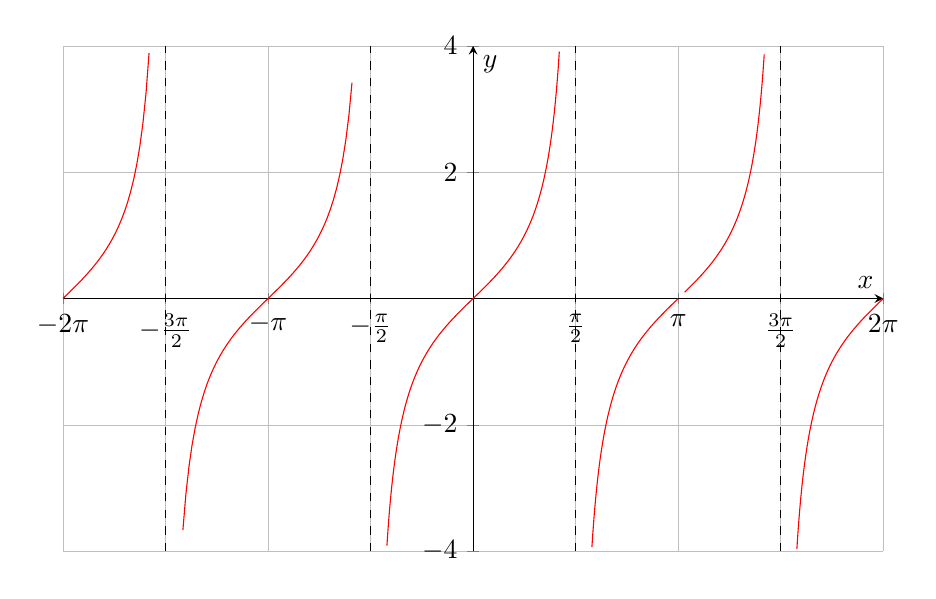
\begin{tikzpicture}
        \begin{axis}[
            axis lines = middle,
            xlabel = $x$,
            ylabel = $y$,
            xmin = -2*pi, xmax = 2*pi,
            ymin = -4, ymax = 4,
            xtick = {-6.28318, -4.71238, -3.14159, -1.5708, 0, 1.5708, 3.14159, 4.71238, 6.28318},
            xticklabels = {$-2\pi$, $-\frac{3\pi}{2}$, $-\pi$, $-\frac{\pi}{2}$, $0$, $\frac{\pi}{2}$, $\pi$, $\frac{3\pi}{2}$, $2\pi$},
            ytick = {-4, -2, 0, 2, 4},
            grid = both,
            grid style = {line width=.1pt, draw=gray!10},
            major grid style = {line width=.2pt,draw=gray!50},
            width = 12cm,
            height = 8cm,
            restrict y to domain=-4:4,
        ]
        \addplot[red, domain=-2*pi:-1.62, samples=100] {tan(deg(x))};
        \addplot[red, domain=-1.52:0, samples=100] {tan(deg(x))};
        \addplot[red, domain=0:1.52, samples=100] {tan(deg(x))};
        \addplot[red, domain=1.62:3.14, samples=100] {tan(deg(x))};
        \addplot[red, domain=3.24:4.66, samples=100] {tan(deg(x))};
        \addplot[red, domain=4.76:6.28, samples=100] {tan(deg(x))};
        
        % Asymptotes verticales
        \addplot[dashed] coordinates {(-4.71238, -4) (-4.71238, 4)};
        \addplot[dashed] coordinates {(-1.5708, -4) (-1.5708, 4)};
        \addplot[dashed] coordinates {(1.5708, -4) (1.5708, 4)};
        \addplot[dashed] coordinates {(4.71238, -4) (4.71238, 4)};
        \end{axis}
    \end{tikzpicture}

    \begin{tikzpicture}
        \begin{axis}[
            axis lines = middle,
            xlabel = $x$,
            ylabel = $y$,
            xmin = -10, xmax = 10,
            ymin = -2, ymax = 2,
            xtick = {-10, -5, 0, 5, 10},
            ytick = {-1.57079, 0, 1.57079},
            yticklabels = {$-\frac{\pi}{2}$, $0$, $\frac{\pi}{2}$},
            grid = both,
            grid style = {line width=.1pt, draw=gray!10},
            major grid style = {line width=.2pt,draw=gray!50},
            width = 12cm,
            height = 8cm,
        ]
        \addplot[blue, domain=-10:10, samples=200] {rad(atan(x))};
        
        % Asymptotes horizontales
        \addplot[dashed] coordinates {(-10, 1.57079) (10, 1.57079)};
        \addplot[dashed] coordinates {(-10, -1.57079) (10, -1.57079)};
        \end{axis}
    \end{tikzpicture}
\end{definition}

\begin{proprietes}
    $\forall x \in ]-1, 1[, (\arctan(x))' = \dfrac{1}{1+x^2}$
\end{proprietes}

\subsection{Fonctions hyperboliques inverses}

$e^ix = \cos(x) + i\sin(x) \iff \cos(x) = \dfrac{e^{ix} + e^{-ix}}{2} \iff \sin(x) = \dfrac{e^{ix} - e^{-ix}}{2}$

\begin{definition}
    On définit par $x \in \R$, le cosinus hyperbolique comme ($\cosh$ ou ch) \linebreak $\cosh(x) = \dfrac{e^x+e^{-x}}{2}$

    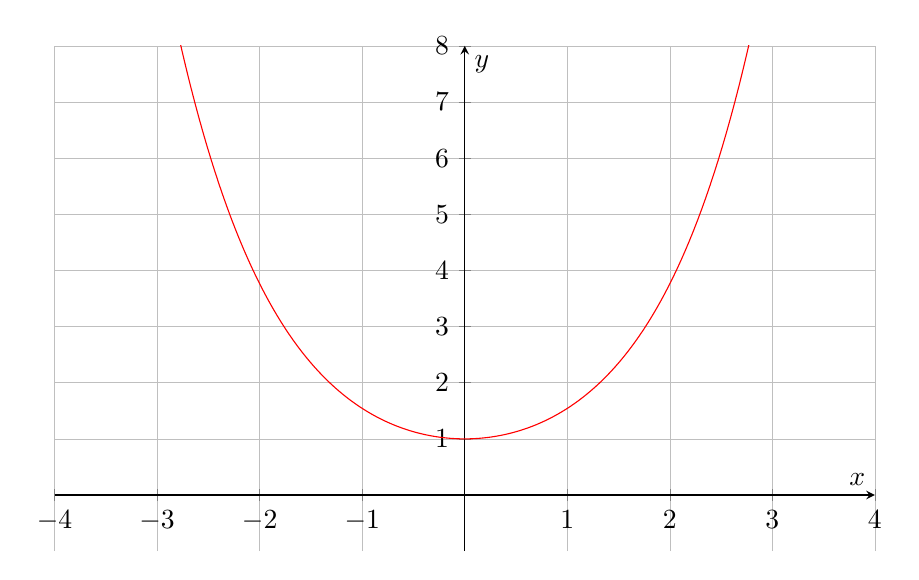
\begin{tikzpicture}
        \begin{axis}[
            axis lines = middle,
            xlabel = $x$,
            ylabel = $y$,
            xmin = -4, xmax = 4,
            ymin = -1, ymax = 8,
            xtick = {-4, -3, -2, -1, 0, 1, 2, 3, 4},
            ytick = {0, 1, 2, 3, 4, 5, 6, 7, 8},
            grid = both,
            grid style = {line width=.1pt, draw=gray!10},
            major grid style = {line width=.2pt,draw=gray!50},
            width = 12cm,
            height = 8cm,
        ]
        \addplot[red, domain=-4:4, samples=200] {(exp(x) + exp(-x))/2};
        \end{axis}
    \end{tikzpicture}

    La fonction $\cosh: [0, +\infty[ \rightarrow [1, +\infty[$ est strictement croissante et continue,
    elle définit une bijection et sa réciproque $\arg\cosh: [1, +\infty[ \rightarrow [0, +\infty[$

    $\arg\cosh(\cosh(x)) = x$ et $\cosh(\arg\cosh(x)) = x$

    \begin{tikzpicture}
        \begin{axis}[
            axis lines = middle,
            xlabel = $x$,
            ylabel = $y$,
            xmin = -1, xmax = 5,
            ymin = -0.5, ymax = 3,
            xtick = {1, 2, 3, 4, 5},
            ytick = {0, 1, 2, 3},
            grid = both,
            grid style = {line width=.1pt, draw=gray!10},
            major grid style = {line width=.2pt,draw=gray!50},
            width = 12cm,
            height = 8cm,
        ]
        \addplot[red, domain=1:5, samples=200] {ln(x + sqrt(x^2 - 1))};
        
        % Asymptote verticale
        \addplot[dashed] coordinates {(1, -0.5) (1, 3)};
        \end{axis}
    \end{tikzpicture}
\end{definition}

\begin{definition}
    On définit par $x \in \R$, le sinus hyperbolique comme ($\sinh$ ou sh) \linebreak $\cosh(x) = \dfrac{e^-+e^{-x}}{2}$

    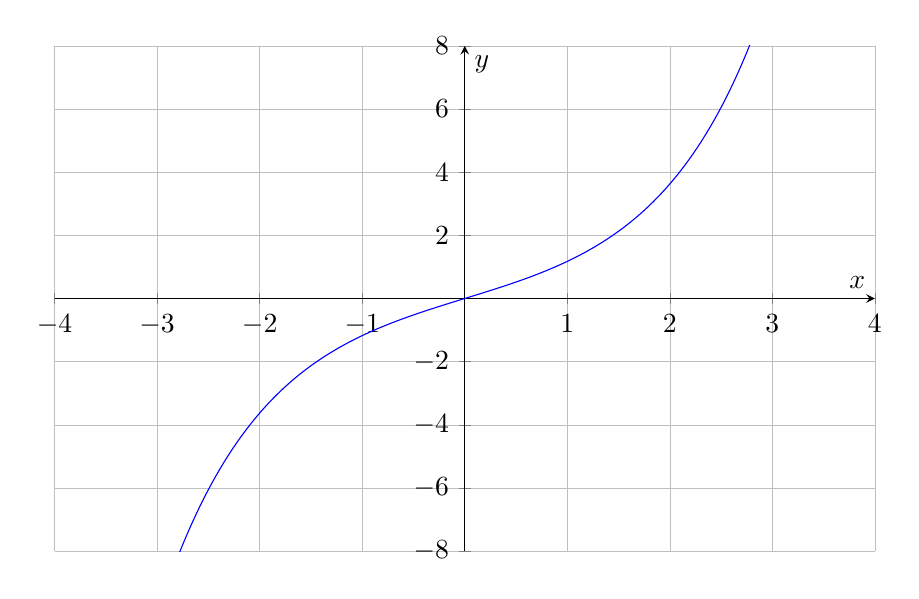
\begin{tikzpicture}
        \begin{axis}[
            axis lines = middle,
            xlabel = $x$,
            ylabel = $y$,
            xmin = -4, xmax = 4,
            ymin = -8, ymax = 8,
            xtick = {-4, -3, -2, -1, 0, 1, 2, 3, 4},
            ytick = {-8, -6, -4, -2, 0, 2, 4, 6, 8},
            grid = both,
            grid style = {line width=.1pt, draw=gray!10},
            major grid style = {line width=.2pt,draw=gray!50},
            width = 12cm,
            height = 8cm,
        ]
        \addplot[blue, domain=-4:4, samples=200] {(exp(x) - exp(-x))/2};
        \end{axis}
    \end{tikzpicture}

    La fonction $\sinh: \R \rightarrow \R$ est continue,
    elle définit une bijection et sa réciproque $\arg\sinh: \R \rightarrow \R$

    $\arg\sinh(\sinh(x)) = x$ et $\sinh(\arg\sinh(x)) = x$

    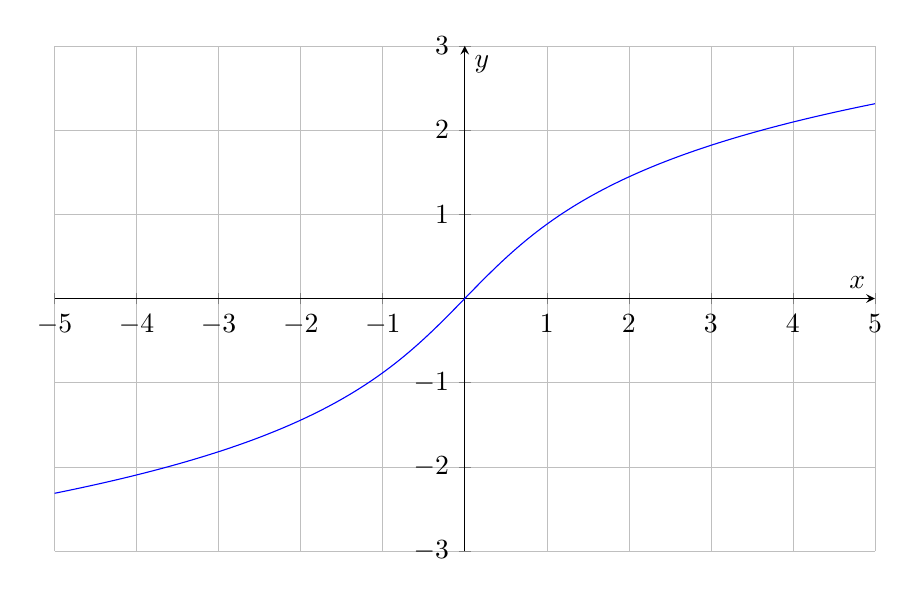
\begin{tikzpicture}
        \begin{axis}[
            axis lines = middle,
            xlabel = $x$,
            ylabel = $y$,
            xmin = -5, xmax = 5,
            ymin = -3, ymax = 3,
            xtick = {-5, -4, -3, -2, -1, 0, 1, 2, 3, 4, 5},
            ytick = {-3, -2, -1, 0, 1, 2, 3},
            grid = both,
            grid style = {line width=.1pt, draw=gray!10},
            major grid style = {line width=.2pt,draw=gray!50},
            width = 12cm,
            height = 8cm,
        ]
        \addplot[blue, domain=-5:5, samples=200] {ln(x + sqrt(1 + x^2))};
        \end{axis}
    \end{tikzpicture}
\end{definition}

\begin{definition}
    On définit par $x \in \R$, la tangente hyperbolique comme ($\tanh$ ou th) \linebreak $\tanh(x) = \dfrac{e^x-e^{-x}}{e^x+e^{-x}}$

    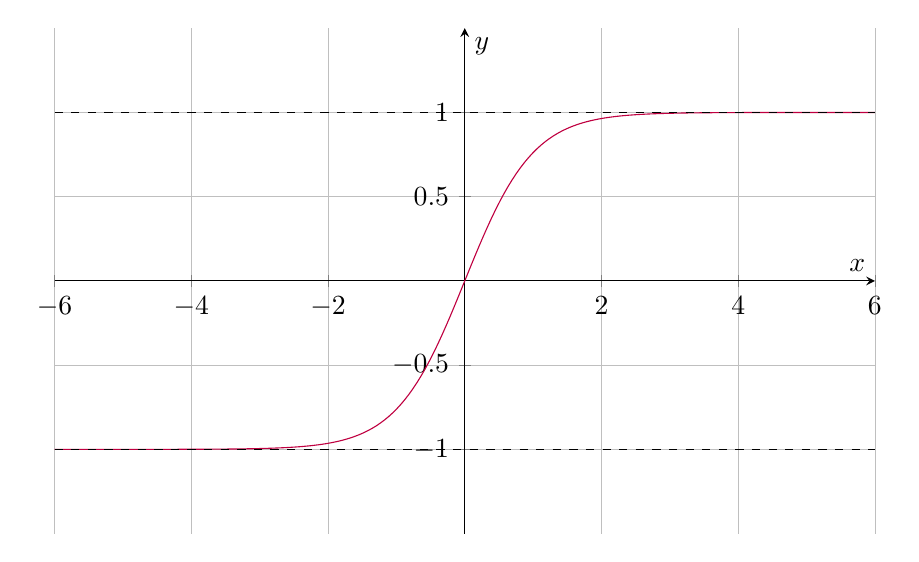
\begin{tikzpicture}
        \begin{axis}[
            axis lines = middle,
            xlabel = $x$,
            ylabel = $y$,
            xmin = -6, xmax = 6,
            ymin = -1.5, ymax = 1.5,
            xtick = {-6, -4, -2, 0, 2, 4, 6},
            ytick = {-1, -0.5, 0, 0.5, 1},
            grid = both,
            grid style = {line width=.1pt, draw=gray!10},
            major grid style = {line width=.2pt,draw=gray!50},
            width = 12cm,
            height = 8cm,
        ]
        \addplot[purple, domain=-6:6, samples=200] {(exp(x) - exp(-x))/(exp(x) + exp(-x))};
        
        % Asymptotes horizontales
        \addplot[dashed] coordinates {(-6, 1) (6, 1)};
        \addplot[dashed] coordinates {(-6, -1) (6, -1)};
        \end{axis}
        \end{tikzpicture}

    La fonction $\tanh: \R \rightarrow ]-1, 1[$ est continue,
    elle définit une bijection et sa réciproque $\arg\tanh: ]-1, 1[ \rightarrow \R$

    $\arg\tanh(\tanh(x)) = x$ et $\tanh(\arg\tanh(x)) = x$

    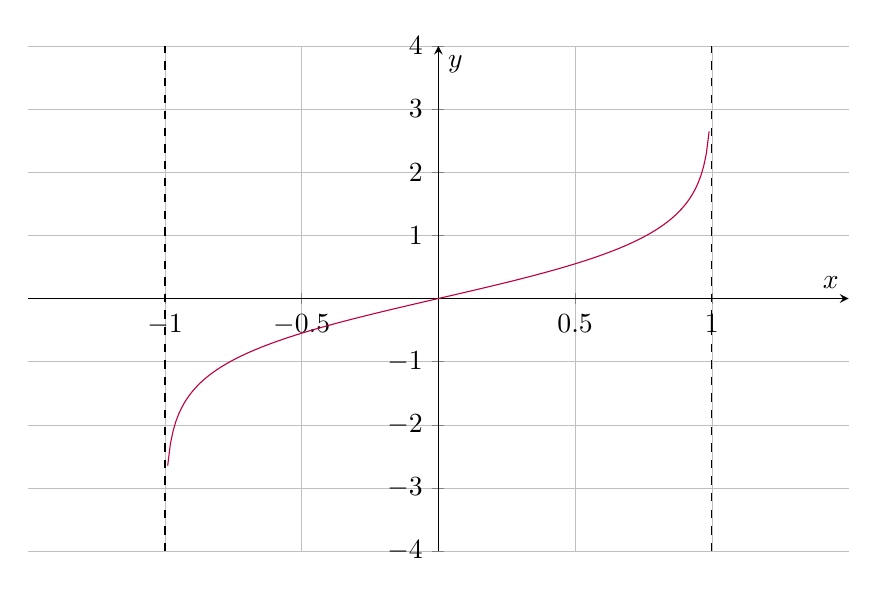
\begin{tikzpicture}
        \begin{axis}[
            axis lines = middle,
            xlabel = $x$,
            ylabel = $y$,
            xmin = -1.5, xmax = 1.5,
            ymin = -4, ymax = 4,
            xtick = {-1, -0.5, 0, 0.5, 1},
            ytick = {-4, -3, -2, -1, 0, 1, 2, 3, 4},
            grid = both,
            grid style = {line width=.1pt, draw=gray!10},
            major grid style = {line width=.2pt,draw=gray!50},
            width = 12cm,
            height = 8cm,
        ]
        \addplot[purple, domain=-0.99:0.99, samples=200] {0.5*ln((1+x)/(1-x))};
        
        % Asymptotes verticales
        \addplot[dashed] coordinates {(-1, -4) (-1, 4)};
        \addplot[dashed] coordinates {(1, -4) (1, 4)};
        \end{axis}
    \end{tikzpicture}
\end{definition}

\begin{proprietes}
    \begin{enumerate}
        \item $(\cosh(x))^2 - (\sinh(x)^2) = 1$
        \item \begin{itemize}
            \item $\cosh(a+b) = \cosh(a) \cosh(b) + \sinh(a) \sinh(b)$
            \item $\cosh(2a) = \cosh(a)^2 + \sinh(a)^2 = 2 \cosh(a)^2 - 1 = 1 + 2 \sinh(a)^2$
            \item $\sinh(a+b) = \sinh(a)\cosh(b) + \sinh(b)\cosh(a)$
            \item $\sinh(2a) = 2\sinh(a)\cosh(b)$
            \item $\tanh(a+b) = \dfrac{\tanh(a) \tanh(b)}{1 + \tanh(a) \tanh(b)}$
        \end{itemize}
        \item \begin{itemize}
            \item $(\cosh(x))' = \sinh(x)$
            \item $(\sinh(x))' = \cosh(x)$
            \item $(\tanh(x))' = 1 - \tanh(x)^2 = \dfrac{1}{\cosh(x)^2}$
        \end{itemize}
    \end{enumerate}
\end{proprietes}


% End of 2024-11-28-CM-11.tex

% Begin of 2024-12-05-CM-12.tex

%verifier les sections
\section{Dérivée d'une fonction}

% retrouver sur internet
equation $y = ax + b = (x - x_0)f'(x_0) + f(x_0) = f'(x_0)x + (f(x_0) - x_0f'(x_0))$

\begin{definition}
    Soit $f: I \R \R$, où I est un interval ouvert de $\R$.
    Soit $x_0 \in I$, on dit que f est dérivable en $x_0$ si le taux d'accroissements
    $\dfrac{f(x)-f(x_0)}{x - x_0}$ admet une limite lorsque x tend vers $x_0$,
    et on la note $\lim_{x \to x_0}\dfrac{f(x) - f(x_0)}{x - x_0} = f'(x_0)$.

    $$
    \forall \eps \gt 0, \exists \delta \gt 0 \text{ alors } |\dfrac{f(x) - f(x_0)}{x - x_0} - f'(x_0)| \lt \eps \iff |f(x) - f(x_0) - (x - x_0)f'(x_0)| \lt \eps |x - x_0| \iff |f(x) - (f(x_0) + (x - x_0)f'(x_0))| \lt \eps |x - x_0|
    $$
\end{definition}

\begin{definition}
    La fonction est dérivable sur I si f est dérivable en tout point x de I.
    On note la fonction $f': \substack{I \R \R \\ x \mapsto f'(x)}$ (parfois $\dfrac{df}{dx}$)
\end{definition}

\begin{proposition}
    \begin{enumerate}
        \item f est dérivable en $x_0$ si et seulement si $\lim_{h \to 0}\dfrac{f(x_0 + h)- f(x_0)}{h}$ existe et est finie.
        \item f est dérivable en $x_0$ ssi il existe un nombre réel $f'(x_0)$ et une fonction $\eps: I \R \R$ avec
        $\eps(x) \to 0$ %mettre une petit x tend vers x_0 sous la flèche
        tel que $f(x) = f(x_0) + f'(x_0)(x - x_0) + \eps(x)(x-x_0)$
    \end{enumerate}
\end{proposition}
%regarder les approximation d'ordre 0, 1 et 2

\begin{demonstration}
    On pose $x = x_0 + h \Rightarrow x - x_0 = h$
\end{demonstration}

\begin{definition}
    La droite qui passe par les points $(x_0, f(x_0))$ et $(x, f(x))$ admet par coefficient directeur $\dfrac{f(x) - f(x_0)}{x - x_0}$.

    A la limite $x \rightarrow x_0$ on trouve le coefficient directeur de la tangente qui vaut $f'(x_0)$ et l'équation de la tangente au point
    $(x_0, f(x_0))$ est donné par $y = (x - x_0)f'(x_0) + f(x_0)$.
\end{definition}

\subsection{Dérivabilité et continuité}

\begin{proposition}
    \begin{enumerate}
        \item Si f est dérivable en $x_0$, alors f est continue en $x_0$.
        \item Si f est dérivable sur I, alors f est continue sur I.
        \item Si f est dérivable et f' est continue, on dit que f est de class $\phi^1$. %check si c'est bien phi
    \end{enumerate}
\end{proposition}

\begin{demonstration}
    Comme f dérivable en $x_0, \exists \eps: I \rightarrow \R$ avec $\eps(x) \to 0$ %pareil x tend vers x_0
    tel que $f(x) = f(x_0) + (x - x_0)f'(x_0) + \eps(x)(x-x_0)$
    et on veut montrer que $\lim_{x \to x_0}f(x) = f(x_0)$

    Ici $\lim_{x \to x_0}f(x) = \lim_{x \to x_0}f(x_0)+(x - x_0)f'(x_0) + \eps(x)(x - x_0)$
\end{demonstration}

\begin{remark}
    \begin{enumerate}
        \item Si f n'est pas continue, alors f n'est pas dérivable (contraposée).
        \item La réciproque est fausse en général (Exemple la fonction $|x|$ en x = 0)
    \end{enumerate}
\end{remark}

\subsection{Calcul de dérivée}

\subsubsection{Règle de calcul}

\begin{proprietes}
    Soient $f: I \rightarrow \R$ et $g: I \rightarrow \R$ dérivable sur I.
    Alors $\forall x \in I$, on a
    \begin{enumerate}
        \item $(f + g)'(x) = f'(x) + g'(x)$
        \item $\forall \lambda \in \R (\lambda f)'(x) = \lambda f'(x)$
        \item $(fg)'(x) = f'(x)g(x) + f(x)g'(x)$
        \item Si $g(x) \neq 0, (\dfrac{f}{g})'(x) = \dfrac{f'(x)g(x) - f(x)g'(x)}{g(x)^2}$
    \end{enumerate}
\end{proprietes}

\begin{demonstration}
    Pour 1 et 2, on utilise la définition de la dérivée.
    $$
    \dfrac{(\lambda f + g)(x) - (\lambda f + g)(x_0)}{x - x_0} \\
    = \dfrac{\lambda f(x) + g(x) - \lambda f(x_0) - g(x_0)}{x - x_0} \\
    = \dfrac{(\lambda f(x) - \lambda f(x_0)) + (g(x) - g(x_0))}{x - x_0} \\
    = \lambda (\dfrac{f(x) - f(x_0)}{x - x_0}) + \dfrac{g(x) - g(x_0)}{x - x_0}
    $$
    %overfull here
    
    Pour 3, on cherche
    $(fg)'(x_0) = \lim_{x \to x_0}\dfrac{fg(x) - fg(x_0)}{x - x_0}$.
    
    $$
    \dfrac{(fg)(x) - (fg)(x_0)}{x - x_0} = \dfrac{f(x)g(x) - f(x_0)g(x_0) + f(x_0)g(x) - f(x_0)g(x_0)}{x - x_0} \\
    = %TODO
    $$
    
    Flemme
\end{demonstration}

\subsubsection{Dérivée de fonctions usuelles}

% A revoir
\begin{methode}
    \begin{enumerate}
        \item $f(x) = x^n \Rightarrow f'(x) = nx^{n-1}$
        \item $f(x) = \dfrac{1}{x} \Rightarrow f'(x) = -\dfrac{1}{x^2}$
        \item $f(x) = \sqrt{x} \Rightarrow f'(x) = \dfrac{1}{2\sqrt{x}}$
        \item $f(x) = e^x \Rightarrow f'(x) = e^x$
        \item $f(x) = a^x \Rightarrow f'(x) = a^x\ln(a)$
        \item $f(x) = \ln(x) \Rightarrow f'(x) = \dfrac{1}{x}$
        \item $f(x) = \log_a(x) \Rightarrow f'(x) = \dfrac{1}{x\ln(a)}$
        \item $f(x) = \sin(x) \Rightarrow f'(x) = \cos(x)$
        \item $f(x) = \cos(x) \Rightarrow f'(x) = -\sin(x)$
        \item $f(x) = \tan(x) \Rightarrow f'(x) = \dfrac{1}{\cos^2(x)}$
    \end{enumerate}
\end{methode}

\subsubsection{Composition}

\begin{proposition}
    Si f dérivable en x et g dérivable en f(x), alors $g \circ f$ est dérivable en x et $(g \circ f)'(x) = g'(f(x))f'(x)$.
\end{proposition}

\begin{demonstration}
    À faire
\end{demonstration}

\begin{corollaire}
    $f: I \rightarrow J$ bijective et dérivable et $f^{-1}: J \rightarrow I$ sa réciproque.
    Si f' ne s'annule pas, alors $f^{-1}$ est dérivable et $(f^{-1})'(x) = \dfrac{1}{f'(f^{-1}(x))}$, $\forall x \in I$
\end{corollaire}

\begin{demonstration}
    À faire
\end{demonstration}

\subsubsection{Dérivées succesives}

Par récurrence, on définit la dérivée n-ième, notée $f^{(n)}$, comme
$f^{(0)} = f, f^{(1)} = f', f^{(n+1)} = (f^{(n)})'$.

Si les dérivées jusqu'à l'ordre n sont définies, on dit que f est de classe $\phi^n$.

\begin{definition}[Formule de Leibniz]
    $(fg)^{(n)}(x) = (f(x)g(x))^{(n)}$
\end{definition}

\begin{definition}[binome de Newton]
    $(a + b)^n = \sum_{k=0}^{n}\binom{n}{k}a^{n-k}b^k$
    À faire
\end{definition}




% End of 2024-12-05-CM-12.tex



\end{document}
